Neste cap�tulo ser�o introduzidos conceitos abordados no decorrer do trabalho.

\section{Computa��o em Nuvem}
Computa��o em nuvem � um modelo elaborado para disponibilizar acesso conveniente, ub�quo e sob demanda via rede a um conjunto compartilhado de recursos computacionais (redes, servidores, armazenamento, aplica��es e servi�os) que possa ser rapidamente alocado e disponibilizado com pouco esfor�o para ger�ncia e m�nima intera��o com provedores de servi�o \cite{nist}.

Em CN, existem tr�s modelos de fornecimento de servi�os que podem ser adotados \cite{nist}, sendo eles:

\begin{itemize}
	\item \textit{Software as a service} \abreviatura{SaaS}{\textit{Software as a Service}}(SaaS): � fornecido aos consumidores a capacidade de executar programas de provedores na infraestrutura da nuvem. Estas aplica��es podem ser acessadas atrav�s de interfaces leves, tais como navegadores. O consumidor n�o despende recursos com a ger�ncia e manuten��o da infraestrutura da nuvem, tais como sistema operacional, redes, servidores ou mesmo configura��es individuais da aplica��o a n�o ser configura��es de execu��o espec�ficas para usu�rio;

	\item \textit{Platform as a service} \abreviatura{PaaS}{\textit{Platform as a Service}}(PaaS): o consumidor do recurso em nuvem possui a capacidade de publicar nesta, aplica��es criadas a partir de linguagens de programa��o, bibliotecas, servi�os e ferramentas suportadas pelo provedor. O cliente n�o gerencia nem tem controle sobre a infraestrutura da nuvem, incluindo a rede, servidores, sistema operacional e armazenamento. Entretanto, ele tem controle das suas aplica��es e possivelmente configura��es sobre o ambiente em que � executada a aplica��o;

	\item \textit{Infrastructure as a service} \abreviatura{IaaS}{\textit{Infrastructure as a Service}}(IaaS): o cliente tem a possibilidade de alocar processamento, armazenamento, servi�os de rede e outros recursos computacionais onde � poss�vel publicar e executar software arbitr�rio, o que pode incluir sistemas operacionais. O consumidor n�o tem a liberdade de gerenciar a infraestrutura f�sica, com exe��o de manter controle sobre armazenamento e suas aplica��es publicadas. Pode existir tamb�m casos em que o consumidor tem controle de componentes espec�ficos da rede, tais como firewall.
\end{itemize}

Este trabalho tem como alvo as nuvens que proveem o servi�o de IaaS. Dessa forma, dado que esse tipo de nuvem deve dividir l�gicamente sua carga de trabalho a fim de atender seus consumidores, deve existir a preocupa��o em segmentar e realocar os recursos de forma eficiente, reduzindo a quantidade de servidores excedentes.


\subsection{Virtualiza��o}
Segundo \citeonline{tholeti2011hypervisors}, virtualiza��o � definida como a cria��o de substitutos para os verdadeiros recursos f�sicos podendo ser criados a partir de divis�es l�gicas. Estes possuem a mesma fun��o e interfaces dos recursos f�sicos, mas diferem em tamanho, performance e custo. Os usu�rios destes recursos virtuais t�picamente n�o percebem a substitui��o, uma vez que sistemas virtuais devem obter performance semelhante a sua contraparte f�sica, em rela��o �s aplica��es dentro do servidor. Usando virtualiza��o � poss�vel fazer com que um recurso f�sico seja visto como m�ltiplos recursos virtuais. A Figura \ref{fig:virtualizacao} demonstra a cria��o de m�ltiplos sistemas virtuais independentes, que usam recursos virtuais, sobre um �nico sistema f�sico.

\begin{figure}[!htb]
 	\centering
 	\caption{Apresenta��o de um ambiente virtualizado, obtido de \cite{tholeti2011hypervisors}.}\label{fig:virtualizacao}
 	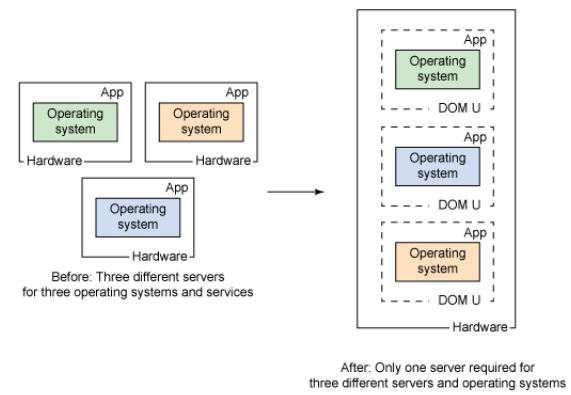
\includegraphics[width=1\textwidth]{figuras/virtualizacao.png}
\end{figure}


Os virtualizadores s�o componentes de software ou firmware capazes de virtualizar recursos f�sicos. Existem tr�s tipos de virtualiza��o diferentes, suas defini��es segundo \citeonline{tholeti2011hypervisors} s�o:

\begin{itemize}
	\item Tipo 1: a virtualiza��o de tipo 1 � caracterizada quando o virtualizador � executado diretamente sobre o hardware do sistema. Este m�todo � mais eficiente, tendo o melhor desempenho entre os m�todos de virtualiza��o;

	\item Tipo 2: a virtualiza��o de tipo 2 � caracterizada quando o virtualizador � executado sobre um sistema operacional hospedeiro que providencia servi�os de virtualiza��o, tais como suporte � entrada/sa�da de dados e gerenciamento de mem�ria;

	\item Virtualiza��o por uso de containers: este modo de virtualiza��o � caracterizado pela abstin�ncia do virtualizador. A virtualiza��o ocorre a n�vel de sistema operacional\abreviatura{SO}{Sistema Operacional} (SO), o qual permite a virtualiza��o de inst�ncias suas. Este modo de virtualiza��o resulta num uso mais eficiente de mem�ria, sendo esta sua vantagem diante dos outros m�todos de virtualiza��o. Todavia, como todas inst�ncias virtuais s�o imagens do SO ra�z, todas as inst�ncias ser�o da mesma vers�o que o SO ra�z.

\end{itemize}

A virtualiza��o � um processo utilizado nos ambientes na nuvem para dividir l�gicamente os recursos f�sicos de um servidor, normalmente sendo usados virtualizadores como componente respons�vel pela cria��o, remo��o e gerenciamento das \textit{virtual machines} \abreviatura{VM}{\textit{Virtual Machine}}(VMs), em portugu�s, m�quinas virtuais. O uso de virtualizadores facilita o provisionamento de diferentes sistemas operacionais sem que eles estejam instalados diretamente nos servidores f�sicos. Outra vantagem da virtualiza��o est� na facilita��o do processo de migra��o de VMs em tempo de execu��o para outros servidores fisicos, facilitando o processo de manuten��o.


\subsection{Efici�ncia energ�tica e consolida��o}
Melhorar a efici�ncia energ�tica � uma das maiores dificuldades da computa��o em nuvem \cite{challenges}, sendo estimado que 53\% de todos os gastos de centro de processamento de dados s�o voltados a energia e refrigera��o \cite{micro-slice}. Aderindo a tend�ncias globais de busca de abordagens sustent�veis, surgiu a ideia de se buscar novas formas de diminuir o consumo de energia em ambientes de computa��o em nuvem, mantendo suporte a cargas din�micas e qualidade de servi�o.

Uma das estrat�gias encontradas para uma melhor efici�ncia energ�tica � a consolida��o. Assim como em \citeonline{gabriel}, no �mbito deste trabalho, consolida��o ser� tratada como a agrega��o de m�quinas virtuais em servidores f�sicos, de forma a concentrar um n�mero maior de m�quinas virtuais em um n�mero menor de servidores f�sicos. Essa forma de agrega��o permite a desativa��o de recursos ociosos, levando a um menor consumo energ�tico.

O benef�cio de t�cnicas de consolida��o vem na possibilidade de aumentar a efici�ncia de um ambiente de CN atrav�s do desligamento de recursos ociosos. Em um cen�rio �timo, todos os servidores que est�o ligados, tendem a carga m�xima, fazendo com que a efici�ncia deste ambiente tamb�m esteja tendendo ao m�ximo poss�vel. Para que seja poss�vel a consolida��o, deve ser poss�vel migrar VMs em tempo de execu��o, fato que s� ocorre entre servidores com hardware compat�vel e mesmo virtualizador. Este e outros fatores, como a necessidade de atender a cargas estoc�sticas, faz com que a consolida��o de ambientes em nuvem n�o seja um problema trivial de se resolver.\par

Para que a consolida��o seja poss�vel, deve haver alguma forma de comunica��o entre servidores, para que estes acordem em realizar um rebalanceamento de carga. Al�m disso, a comunica��o e migra��o deve ocorrer entre m�quinas que se encaixam no cen�rio em que h� a necessidade de uma migra��o em tempo de execu��o. Neste tipo de ambiente, al�m de estarem presentes conceitos de negocia��o e atos de fala, h� informa��o fragmentada inserida nos elementos do ambiente. Tais pontos s�o discutidos e est�o presentes no conjunto de caracter�sticas de problemas onde o uso de sistemas multiagente � recomendado, apontadas por Wooldridge em seu livro \cite{wooldridge2009introduction}.


\subsection{Orquestra��o}
Dadas a complexidade e heterogeneidade de ambientes de computa��o em nuvem, contendo in�meros componentes e vari�veis din�micas interligadas, a ger�ncia destes ambientes torna-se humanamente imposs�vel\\ \cite{forecasting}. Tendo isso em vista, ferramentas foram criadas com o objetivo de orquestrar a infraestrutura do ambiente, realizando a liga��o dos diferentes componentes como servidores de armazenamento, virtualiza��o e dispositivos de redes para prover a abstra��o de uma nuvem computacional.

\citeonline{gabriel} cita cinco componentes que comp�em as ferramentas dispon�veis para orquestra��o:
\begin{enumerate}
 \item Um gerente de identidades que realiza a ger�ncia das credenciais dos usu�rios (autentica��o e autoriza��o), possibilitando seguran�a na organiza��o da infraestrutura;
 \item Um gerente de aloca��o que aloca m�quinas virtuais quando s�o instanciadas, ligadas ou migradas;
 \item Um \emph{hypervisor} que � o componente que interage com diferentes virtualizadores, sendo respons�vel por enviar comandos para cada cluster;
 \item Um componente de armazenamento que realiza a distribui��o e o compartilhamento das unidades de armazenamento de m�quinas virtuais entre os servidores;
 \item Um elemento encarregado de gerenciar a configura��o da rede.
\end{enumerate}

A Figura \ref{fig:orquestracao}, retirada de \citeonline{gabriel}, apresenta um modelo gen�rico de ferramenta de orquestra��o.

 \begin{figure}[!htb]
 	\centering
 	\caption{Modelo de uma ferramenta de orquestra��o \cite{gabriel}.}\label{fig:orquestracao}
 	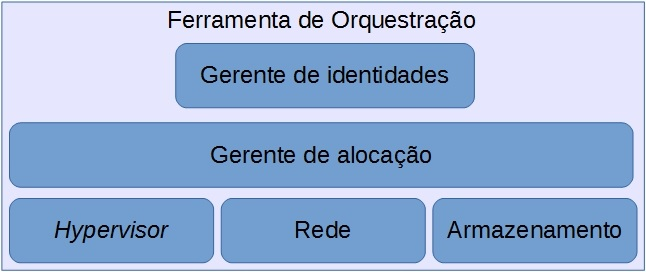
\includegraphics[scale=0.45]{figuras/ferramentasOrquestracao.jpg}
 \end{figure}

A ferramenta escolhida por \citeonline{gabriel}, que tamb�m ser� utilizada nesse trabalho, � o \textit{Cloudstack} \cite{cloudstack}. A escolha � motivada pelos fatos de que a ferramenta demonstra uma evolu��o constante num projeto que mant�m uma comunidade participativa, documenta��o completa e detalhada e o uso de tecnologias conhecidas para armazenamento de dados.


\section{Sistemas Multiagentes}
Sistemas multiagentes � considerada uma �rea de estudo dentro da Intelig�ncia Artificial Distribu�da (IAD)\abreviatura{IAD}{Intelig�ncia Artificial Distribu�da}. SMA possuem a capacidade de lidar com problemas em ambientes distribu�dos e abertos, tal como os ambientes em larga escala encontrados que usam a internet como meio \cite{wooldridge2009introduction}.\par

A abordagem de SMA � descrita na forma de m�ltiplos elementos computacionais (agentes) que trocam conhecimento entre si na forma de coopera��o, coordena��o, negocia��o e similares, possibilitando a fragmenta��o de problemas complexos em sub-problemas menores e objetivos. Estes, por sua vez, podem ser abordados de diferentes formas, por diferentes agentes especialistas \cite{a-ricardo-intro}.\par

O emprego de SMA tem apresentado sucesso em �reas que trabalham com ambientes din�micos e descentralizados, onde a tomada de decis�o n�o depende apenas de um �nico ponto de vista \cite{kelash2007takes}.

\subsection{Agentes}
% LUCAS

 Agentes s�o entidades capazes de se comunicar entre si, possuem mobilidade e comportam-se de forma independente e inteligente dentro do ambiente. Um agente � um sistema computacional capaz de atuar autonomamente de maneira a alcan�ar seus objetivos \cite{wooldridge2009introduction}. Seu conceito pode ser  abstraido para uma entidade auto-contida, capaz de interagir (atrav�s de fun��es atuadoras e sensoras) com o 
ambiente em que se encontra, consigo mesma e com outros agentes \cite{ia-ferramentas}. Ter v�rios agentes em um sistema implica que cada agente deve raciocinar e agir levando em considera��o os outros agentes no sistema, sendo que dentro de um sistema, diferentes agentes podem ou n�o ter um prop�sito em comum \cite{handbook-knowledge}. Este segundo caso � particularmente interessante, j� que as diferentes entidades podem ter o mesmo objetivo, mas diferentes crit�rios, possivelmente conflitantes, a priorizar na satisfa��o de suas metas. Independente de seu tipo e ambiente, agentes funcionam em um ciclo cont�nuo de perceber o mundo, decidir sua pr�xima a��o e execut�-la. A Figura \ref{fig:agente} representa o ciclo cont�nuo de execu��o de um agente. 

\begin{figure}[!htb]
	\centering
	\caption{Representa��o de um agente em um ambiente, obtido de \cite{RussellLivro}.}\label{fig:agente}
	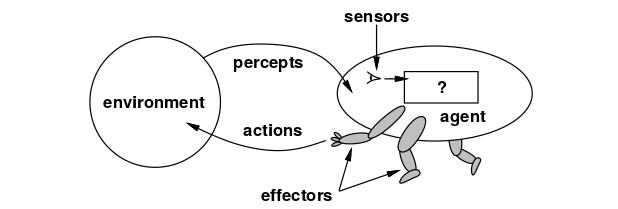
\includegraphics[width=1\textwidth]{figuras/imgAgent.png}
\end{figure}

Agentes possuem m�dulos que servem como sensores e atuadores, representando sua interface com o mundo. Eles est�o diretamente relacionados com as capacidades dos agentes de perceber e agir. Atrav�s dos sensores, um agente consegue perceber o ambiente que ele est� inserido. Esta entrada, na forma percep��es, � avaliada pelo agente, resultando em uma decis�o de a��o. Por fim, atrav�s dos atuadores, o agente � capaz de agir em seu ambiente, modificando o estado do ambiente.

\subsubsection{Caracter�sticas de Agentes}

Um agente � respons�vel por representar um ponto de vista e agir de forma coerente para alcan�ar um objetivo. Assim como uma sociedade de agentes exprime v�rios pontos de vista e objetivos. No evento em que dois ou mais pontos de vista entram em conflito, os agentes devem ter a capacidade de negociar, para que possam encontrar a melhor a��o para o problema em conjunto \cite{wooldridge2009introduction}.\par 

Segundo Silveira em \cite{a-ricardo-intro}, mesmo tendo natureza diversa, os agentes possuem caracter�sticas recorrentes, relacionadas com suas abordagens para resolver problemas e capacidade de comunica��o. Encontrado em maior ou menor grau em uma implementa��o de um agente, estes atributos s�o:

\begin{itemize}  
	\item Reatividade: a habilidade de perceber o ambiente de modo seletivo e manifestar um
	comportamento como resposta a um est�mulo externo;
	\item Autonomia: comportamento dirigido a objetivos, pr�-ativo e auto-iniciado;
	\item Comportamento cooperativo: trabalhar com outros agentes para atingir um objetivo
	comum;
	\item Habilidade de comunica��o ao n�vel de conhecimento: capacidade de comunicar-se com
	pessoas ou outros agentes em uma linguagem de mais alto n�vel que um simples protocolo
	de comunica��o programa a programa;
	\item Capacidade de infer�ncia: capacidade de agir a partir de especifica��es abstratas de
	tarefas, usando conhecimentos pr�vios;
	\item Continuidade temporal: persist�ncia de identidade por longos per�odos de tempo;
	\item Personalidade: capacidade de demonstrar atributos de um personagem;
	\item Adaptabilidade: habilidade de aprender com a experi�ncia;
	\item Mobilidade: habilidade de migrar de uma plataforma para outra.
\end{itemize}

As diferen�as entre agentes � o fator respons�vel pela heterogeniedade do SMA. O fato de que diferentes entidades dividem o mesmo ambiente, faz com que um problema possa ser percebido de diferentes formas e lidado de maneiras diferentes e condizentes com um plano de a��o conjunto. Em adi��o � suas caracter�sticas, os agentes possuem estrat�gias diferentes para a tomada de decis�o, fator que gera diferentes classifica��es para estes, descritas nas pr�ximas sub-se��es.

\subsubsection{Agentes Reativos}

Segundo \citeonline{wooldridge2009introduction}, agentes puramente reativos s�o entidades computacionais que decidem suas a��es baseados exclusivamente no estado presente do ambiente. Eles recebem seu nome em raz�o do comportamento an�logo a uma resposta imediata, sem consulta a um hist�rico passado de conhecimento. Essa abordagem � focada no que os agentes podem realizar, juntos ou separadamente, sem existir necessariamente mem�ria ou comunica��o direta entre eles. Nesse caso, agentes tomam conhecimento de a��es e comportamentos de outros 
agentes apenas atrav�s de modifica��es no ambiente \cite{ia-ferramentas}. Embora sejam �teis em raz�o de que s�o programados de forma a ter comportamentos hierarquicamente organizados, esse tipo de agente pode se tornar muito complexo para entender quando o n�mero de comportamentos associado a eles cresce.

\subsection{Agentes Deliberativos}

Agentes deliberativos s�o aqueles que tem alguma forma de reten��o de conhecimento na forma de experi�ncias passadas, criando um modelo expl�cito de mundo. Estes agentes tamb�m possuem uma expl�cita representa��o de outros agentes, mem�ria (que 
permite que os agentes plenejem suas a��es tendo eventos passados como base) e capacidade de se comunicarem diretamente uns com os outros. Esse modelo de agente � mais focado nas atitudes que os caracterizam, sendo que com o tempo, realizando diferentes intera��es com os sistemas, estes devem desenvolver cren�as (no sentido de reconhecer padr�es), inten��es, entre outras caracter�sticas de uma entidade racional com a finalidade de auxiliar a escolha de seus planos de a��o futuros, suplementando sua percep��o atual do ambiente \cite{handbook-knowledge}.\par

No contexto de um agente cognitivo, um conjunto de cren�as � chamado de banco de conhecimento. Esse � continuamente atualizado com as percep��es do agente, assim como � usado para verificar condi��es necess�rias para a escolha de um pr�ximo plano de a��o do agente. Na Figura \ref{fig:agente-BDI} pode-se observar a arquitetura de um agente deliberativo que age no formato de \textit{Beliefs, Desire and Intentions} \abreviatura{BDI}{Beliefs Desire Intentions}(BDI), em portugu�s cren�as, desejos e inten��es.

\begin{figure}[!htb]
	\centering
	\caption{Modelo gen�rico de um agente deliberativo BDI, obtido de \cite{bdi4jade}.}\label{fig:agente-BDI}
	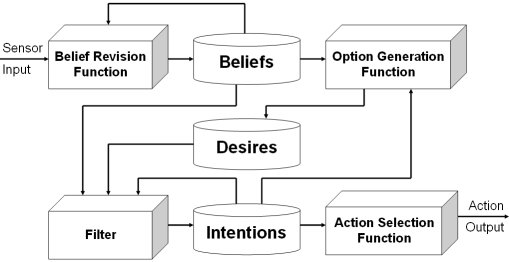
\includegraphics[width=1\textwidth]{figuras/bdiArch.jpg}
\end{figure}

Os agentes BDI s�o aqueles que mant�m uma s�rie de objetivos, armazenados na forma de desejos, mant�m planos na forma de inten��es e possuem cren�as, que s�o informa��es que guardam de forma simb�lica sobre o ambiente. Utilizando l�gica de predicados de primeira ordem, um agente BDI pode escolher qual plano melhor se encaixa na sua vis�o de mundo atual.

\subsubsection{Agentes H�bridos}

De acordo com \cite{wooldridge2009introduction}, agentes h�bridos s�o capazes de apresentar comportamento reativo e proativo atrav�s da modelagem de camadas de comportamentos. A partir dos dados providos pela leitura do ambiente, o agente pondera seus comportamentos da camada de planos reativos e da sua camada de comportamentos proativos. A sa�da dessa fun��o de pondera��o � interpretada de forma an�loga a uma sugest�o de plano. Agentes deste tipo funcionam gra�as a presen�a expl�cita ou n�o de uma camada de controle de comportamentos.

\subsection{Modelagem de Sistemas de Agentes}
Sistemas baseados em agentes podem ser modelados de forma similar a sistemas orientados a objeto, sendo que seus agentes tomam forma de objeto e passam a ser constitu�dos por atributos e m�todos podendo se comunicar invocando m�todos de outros agentes ou trocando mensagens, e podendo utilizar conceitos cl�ssicos de orienta��o a objeto, como heran�a, encapsulamento e agrega��o de dados \cite{intelligent}. Em consequ�ncia disso, m�todos relacionados ao desenvolvimento de aplicativos orientados a objeto formam a base de boa parte dos m�todos de desenvolvimento de sistemas baseados em agentes. De forma similar a t�cnica para modelagem orientada a objeto proposta por \citeonline{OMT} que consiste de modelo b�sico, modelo est�tico e modelo din�mico, \citeonline{agent-oriented} divide a an�lise orientada a agentes em tr�s modelos, o modelo de agente, o modelo organizacional e o modelo cooperativo, descritos a seguir:

\begin{itemize}
  \item O modelo de agente cont�m descri��es e estruturas internas dos agentes, descritas em termos de no��es mentais como metas planos e cren�as ou quaisquer estruturas que sejam apropriadas a arquitetura espec�fica dos agentes sendo desenvolvidos. Esse modelo se assemelha ao modelo b�sico de m�todos de orienta��o a objeto;
  \item O modelo organizacional especifica os relacionamentos entre agentes e seus tipos. Estes s�o em parte rela��es de heran�a, e tamb�m relacionamentos entre agentes baseados em seus respectivos pap�is em organiza��es. Essas organiza��es podem ser meios para estruturar sistemas complexos em subsistemas (assim como � feito em certas t�cnicas de orienta��o a objeto) ou podem ser usadas para modelar organiza��es reais. Esse modelo � semelhante ao modelo est�tico, mas como pap�is podem mudar com o passar do tempo, ele n�o � um modelo genuinamente est�tico;
  \item O modelo cooperativo descreve a intera��o, ou mais especificamente, a coopera��o entre os agentes. Este modelo cont�m apenas os \hyphenation{relacio-namentos} relacionamentos entre objetos. O processo que ocorre dentro dos objetos � representado pelo modelo de agente.
\end{itemize}


\subsection{Comunica��o de Agentes}
A coopera��o e a comunica��o entre agentes torna-se interessante quando existe a inten��o de resolver um problema de forma distribu�da, como � o caso da orquestra��o de um ambiente de computa��o em nuvem. Existem v�rios m�todos de comunica��o entre agentes fundamentalmente diferentes, sendo que \citeonline{intelligent} classificam como o mais simples dos m�todos a invoca��o do procedimento de um agente por outro agente.

Utilizando a invoca��o de procedimentos, o agente invocador (agente 1) usa par�metros de invoca��o expl�citos para informar o outro agente (agente 2) de suas inten��es. Os valores de retorno do agente 2 representam a resposta da comunica��o. Por�m, apenas comunica��es muito simples podem ser efetuadas invocando procedimentos remotos, sendo que para casos com um m�nimo de complexidade os m�todos de comunica��o entre agentes podem ser diferenciados em sistemas \emph{blackboard} (quadro negro) e sistemas baseados em di�logo (troca de mensagens) \cite{intelligent}.

O conceito de quadro negro surgiu a partir da inten��o de lidar com aplica��es complexas e fracamente definidas, dando mais flexibilidade a pesquisadores e desenvolvedores, liberando-os de especifica��es formais excecivas \cite{blackboard}. Um quadro negro proporciona a todos os agentes dentro de um sistema uma �rea comum de trabalho, a qual eles podem utilizar para trocar informa��es \cite{intelligent}. Um agente inicia a comunica��o escrevendo um item de informa��o qualquer no quadro negro. Este item fica ent�o dispon�vel para todos os outros agentes do sistema, sendo que qualquer agente pode acessar o quadro negro a qualquer momento para verificar se novas informa��es surgiram desde sua �ltima verifica��o \cite{intelligent}. Neste modelo os agentes n�o precisam saber dos conhecimentos e nem da exist�ncia dos outros agentes dentro do sistema, mas devem ser capazes de compreender as informa��es contidas no quadro negro \cite{blackboard}.

A alternativa ao quadro negro vem na forma de troca de mensagens. A comunica��o via troca de mensagens proporciona uma base flex�vel para a implementa��o de estrat�gias complexas de coordena��o de agentes, sendo que as mensagens trocadas entre os agentes podem ser usadas para estabelecer comunica��es e mecanismos de coopera��o usando protocolos pr�-definidos \cite{intelligent}. O fato de que diferentes agentes podem ser invocados para realizarem fun��es diferentes dentro do ambiente, mas em algum ponto de suas respectivas fun��es, necessitar de alguma informa��o da qual outro agente pode ter conhecimento \cite{handbook-intelligence} � algo que torna essa abordagem interessante em um ambiente de computa��o em nuvem.


\subsection{Padr�es de Comunica��o}
Com o �mbito de iniciar a padroniza��o das linguagens de sistemas aut�nomos, a \textit{Defense Advanced Research Projects Agency} \abreviatura{DARPA}{\textit{Defense Advanced Research Projects Agency}}(DARPA) \cite{darpasite}, iniciou um movimento chamado de \abreviatura{KSE}{\textit{Knowledge Sharing Effort}}\textit{Knowledge Sharing Effort} (KSE) \cite{ksesite} que mais tarde geraria o primeiro padr�o de mensagens para comunica��o de agentes, o \textit{Knowledge Query and Manipulation Language} \abreviatura{KQML}{\textit{Knowledge Query and Manipulation Language}}(KQML) \cite{finin1994kqml}.\par

O KQML � uma linguagem para comunica��o de agentes, servindo como um envelope sem�ntico para o conte�do da mensagem. O padr�o define um formato comum para as trocas de informa��o entre agentes, sem interferir no conte�do em si. Segundo Wooldridge em \cite{wooldridge2009introduction}, o envelope � composto de par�metros na forma de chave-valor. Estes tem a fun��o de garantir caracter�sticas tais como independ�ncia de linguagem e suporte a diferentes representa��es internas de conhecimento. Dessa forma o receptor pode, entre outras coisas, saber a linguagem em que o remetente escreveu e espera a resposta e ter acesso a ontologia do remetente. Os par�metros da mensagens s�o complementados por um elemento performativo que � an�logo ao tipo da mensagem (ex. pergunta, resposta, oferta, entre outros). Seguindo um racioc�nio similar a orienta��o a objetos, pode-se pensar em performativas como a classe de um objeto mensagem e seus par�metros ( pares chave-valor ) como vari�veis de uma inst�ncia.\par

Atrav�s da padroniza��o de mensagens, agentes podem diferenciar sem�nticamente mensagens que possuem o mesmo conte�do, atrav�s do uso de cabe�alhos distintos. Segundo \cite{wooldridge2009introduction}, o KQML foi criticado, entre outras raz�es, pela aus�ncia de performativas necess�rias para atos de coordena��o entre agentes e por ter sem�ntica pouco rigorosa, levando a mensagens amb�guas. Outros padr�es foram ent�o propostos e introduzidos no cen�rio de comunica��o de agentes.\par

\subsubsection{Especifica��es FIPA}\label{esp-fipa}

A FIPA \abreviatura{FIPA}{\textit{Foundation for Intelligent Physical Agents}}(\emph{Foundation for Intelligent Physical Agents}) � uma organiza��o que promove tecnologia baseada em agentes e a interoperabilidade de seus padr�es com outras tecnologias \cite{fipa}. As v�rias especifica��es promovidas pela FIPA abrangem diferentes categorias, sendo essas:
\begin{itemize}
	\item Comunica��o de Agentes;
	\item Transporte de Agentes;
	\item Gerenciamento de Agentes;
	\item Arquitetura abstrata de agentes;
	\item Aplicativos.
\end{itemize}

Dentre as categorias as quais o padr�o FIPA especifica, \cite{fipa} define comunica��o de agentes como sendo a parte principal de seu modelo de sistema multiagente como um todo. O primeiro documento produzido pela FIPA, chamado FIPA97 \cite{fipa97}, especifica as regras normativas que permitem que uma sociedade de agentes interopere, ou seja, existir, operar e serem gerenciados \cite{jade-fipa}. As regras foram desenvolvidas englobando os preceitos de reusabilidade e interoperabilidade entre SMAs. O padr�o FIPA usa a mesma estrutura proposta pelo KQML, por�m suas cole��es de a��es performativas divergem. A linguagem de comunica��o entre agentes FIPA tem como ponto forte uma sem�ntica baseada em teorias de atos de di�logos mapeados para a��es racionais. Dessa forma, as mensagens podem representar cren�as, vontades e incertezas de um agente de forma n�o amb�gua \cite{serugendo2007autonomous}.\par

Al�m disso, \citeonline{fipa97} tamb�m especifica a \abreviatura{ACL}{\textit{Agent Communcation Language}}ACL (\emph{Agent Communcation Language}), uma linguagem voltada especificamente para a comunica��o entre agentes. A ACL especifica a codifica��o e sem�ntica das mensagens trocadas entre agentes, mas n�o especifica um mecanismo ou t�cnologia a ser usada para a troca de mensagens. Sendo assim, implementa��es usando \textit{Java multi-threads}, \abreviatura{CORBA}{\textit{Common Object Request Broker Architeture}}CORBA, entre outras podem ser utilizadas para aplicar o padr�o FIPA.\par

Em fun��o da diversidade de t�cnologias que as plataformas podem empregar para realizar o transporte de mensagem e de que agentes distintos podem residir em plataformas de terceiros, possivelmente utilizando tecnologias de rede diferentes, a FIPA especifica que mensagens que s�o transportadas entre plataformas desconexas devem ser codificadas em forma de texto \cite{jade-fipa}.\par

� importante ressaltar que o padr�o FIPA, segundo o documento de especifica��es FIPA97, descreve tamb�m o modelo de refer�ncia para plataformas de sistemas multiagentes, sendo identificados agentes e fun��es chaves necess�rios para o controle da plataforma. Os agentes indispens�veis para manuten��o e funcionamento da plataforma, apresentados na Figura \ref{fig:fipa}, s�o:

\begin{figure}[!htb]
	\centering
	\caption{Refer�ncia de plataformas de agente do padr�o FIPA, retirada de \cite{jade-fipa}.}\label{fig:fipa}
	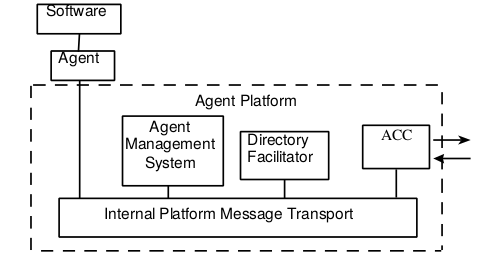
\includegraphics[width=1\textwidth]{figuras/fipa.png}
\end{figure}


\begin{itemize}
	\item \textit{Agent Management System}\abreviatura{AMS}{\textit{Agent Management System}} (AMS) � o agente que deve supervisionar o acesso e uso da plataforma. Ele � respons�vel por autenticar os agentes internos e controlar seus registros;

	\item \textit{Agent Communication Channel}\abreviatura{ACC}{\textit{Agent Communication Channel}} (ACC) � o agente que providencia o caminho para contatos b�sicos entre agentes dentro e fora da plataforma. Ele � o m�todo padr�o de comunica��o que oferece um servi�o confi�vel, preciso e ordenado de mensagens. Este agente deve ser respons�vel tamb�m por trazer suporte para interoperabilidade entre diferentes plataformas de agentes;

	\item \textit{Directory Facilitator}\abreviatura{DF}{\textit{Directory Facilitator}} (DF) � o agente que disp�e um servi�o de p�ginas amarelas � plataforma de agentes.
\end{itemize}

O objetivo dos padr�es desenvolvidos pela FIPA s�o de chegar a um consenso sem que as normas acordadas tornem-se um fator negativo para o desenvolvimento de sistemas multiagentes. Tendo isso em mente a FIPA define apenas o comportamento externo dos sistemas multiagentes, deixando com que o interior desses sistemas possam ser propriet�rios. Tais defini��es n�o se limitam apenas a comunica��o de agentes e podem se extender at� mobilidade, seguran�a e integra��o agente-\textit{software}, sendo estas descritas em detalhe no site da FIPA \cite{fipa}.


\subsection{Ferramentas existentes}
Esta se��o � designada a apresentar as plataformas de SMA mais utilizadas, seus pontos fortes, fracos e caracter�sticas.

\subsubsection{JACAMO}

Jacamo combina tr�s t�cnologias distintas, modulares e consolidadas para formar um \textit{framework} de programa��o de SMA com o objetivo de cobrir todos os n�veis de abstra��o \cite{jacamo}. As t�cnologias que o comp�e s�o:

\begin{enumerate}
	\item \textit{Jason}: usada para programar os agentes aut�nomos \cite{jasonsite}.
	\item \textit{Cartago}: inclu�do para implementar os artefatos que comp�e o ambiente \cite{cartago}.
	\item \textit{Moise}: usado para programar as organiza��es entre os agentes \cite{moise}.
\end{enumerate}

O desenvolvimento envolvendo o \textit{framework} parte do princ�pio que o ambiente � algo end�geno, ou seja este faz parte do sistema a ser desenvolvido. Dessa forma, atrav�s do uso do Cartago, pode-se desenvolver o ambiente enquanto o Jason serve de \textit{framework} para o desenvolvimento de agentes. Assim, o ambiente � exposto para os agentes como uma cole��o de artefatos \cite{jacamo}, como � visto na Figura \ref{fig:jacamo}.

\begin{figure}[!htb]
	\centering
	\caption{Conex�o entre Cartago e Jason no ciclo de desenvolvimento do Jacamo, retirado de \cite{jacamo}.}\label{fig:jacamo}
	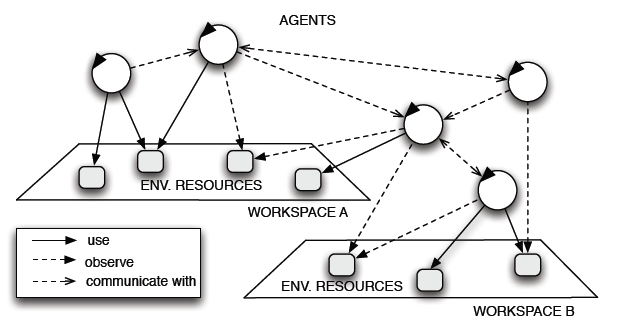
\includegraphics[width=1\textwidth]{figuras/jacamo.png}
\end{figure}

Ap�s o desenvolvimento do ambiente e dos agentes, o componente Moise � respons�vel por criar um meta-modelo organizacional de forma a definir estruturas de grupos de agentes, pap�is e entidades. Este componente tamb�m deve criar especifica��es funcionais atrav�s da defini��o dos objetivos atribu�dos aos agentes, esquemas sociais baseados na agrega��o dos objetivos de organiza��es na forma de miss�es e especifica��es normativas que ligam pap�is a objetivos, delimitando o comportamento do agente quando este assume um pap�l dentro de um grupo.

Embora o jacamo encaixe bem no ambiente proposto por este trabalho, n�o h� men��o sobre sua adaptabilidade a infraestruturas distr�buidas. Este fator deixa a d�vida sobre a capacidade de implementa��o do \textit{framework} sobre infraestruturas n�o centralizadas e tolerante a falhas. Entretanto, o conceito de artefatos e ambientes end�gneos pode ser aproveitado para esta aplica��o, uma vez que os agentes encontram-se exteriorizados � ferramenta de orquestra��o e sua comunica��o � limitada a fun��es espec�ficas, comparadas diretamente aos conceitos de artefatos proposto pelo Cartago.

\subsubsection{JADE}

\textit{Java Agent DEvelopment} \abreviatura{JADE}{\textit{Java Agent Development}}(JADE)\cite{jade} � um \textit{framework} para desenvolvimento de aplica��es de agentes compat�vel com as especifica��es da FIPA para interoperabilidade entre sistemas multiagentes, desenvolvido inicialmente pela Telecom Italia (que, na data deste trabalho, ainda � detentora dos direitos autorais sobre a ferramenta), � distribu�da em formato de c�digo aberto sob as condi��es da LGPLv2 \cite{lgpl2}. O objetivo da ferramenta JADE � providenciar ao desenvolvedor uma maneira simples de desenvolver seu programa, facilitando a implementa��o dos padr�es da FIPA. As caracter�sticas do JADE importantes para o problema apresentado neste trabalho s�o:

\begin{itemize}
	\item Plataforma que segue o padr�o FIPA, incluindo os tr�s agentes necess�rios descritos na se��o \ref{esp-fipa}, ativados junto com a inicializa��o da plataforma;

	\item Plataforma de agentes distribu�da. A plataforma pode ser dividida entre v�rios servidores, contanto que n�o haja \textit{firewall} entre eles, usando apenas uma aplica��o em cada servidor, rodando em uma \textit{Java Virtual Machine}\abreviatura{JVM}{\textit{Java Virtual Machine}} (JVM). Agentes s�o implementados como uma \textit{thread} Java e suas a��es paralelas s�o tratadas como tarefas, estas escalonadas pela pr�pria plataforma de maneira leve e eficiente. A comunica��o entre agentes na mesma JVM se d� pelo uso de \textit{Java Events};

	\item Transporte de mensagens dentro da mesma plataforma � feito atrav�s de transfer�ncias de objetos Java para evitar convers�es de dados. Quando o receptor ou remetente n�o perten�e a mesma plataforma, a mensagem � automaticamente convertida para o formato FIPA;

	\item Suporte a agentes reativos e a agentes BDI a partir de um modelo de agente gen�rico.

\end{itemize}

As JVMs instanciadas atuam, cada uma, como um container de agentes do JADE. Cada container � respons�vel por gerenciar localmente o ciclo de vida de seus agentes instanciados, assim como deve manter as informa��es necess�rias para realizar a comunica��o dos seus agentes com agentes residentes em outros containers, tais como um \textit{buffer} contendo o endere�o de agentes externos cujo foi trocado mensagens recentemente.\par

Uma JVM do JADE ir� assumir o papel de fachada da plataforma para o ambiente externo. Este container especial possui os agentes de ger�ncia descritos pela FIPA e � respons�vel por representar toda a plataforma para com plataformas de SMA de terceiros. Assim, esta inst�ncia � respons�vel, dentre outras coisas, por fazer o roteamento das mensagens trocadas entre agentes internos e externos � plataforma, registro de agentes e descoberta de agentes em outras plataformas. A Figura \ref{fig:jadearq} representa a arquitetura do JADE de forma visual.

\begin{figure}[!htb]
	\centering
	\caption{Arquitetura da plataforma JADE, obtida de \cite{jade-site}.}\label{fig:jadearq}
	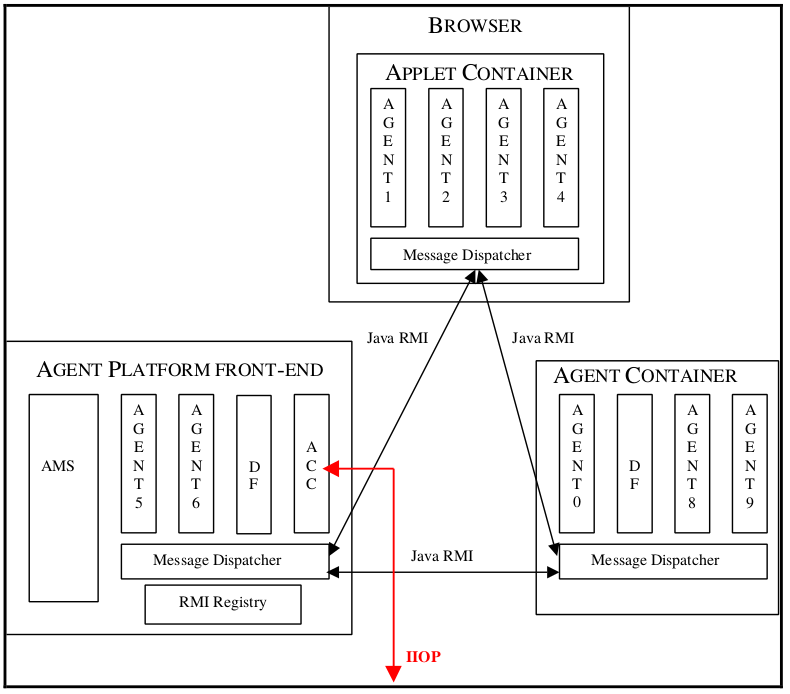
\includegraphics[width=1\textwidth]{figuras/jadearq.png}
\end{figure}

Agentes devem ser capazes de se comunicar com outros agentes tanto dentro da mesma plataforma quanto com agentes externos a esta. Os agentes externos s�o aqueles alocados em outros SMAs fora do dom�nio da aplica��o. Para que a troca de mensagens seja poss�vel, ambas as plataformas devem respeitar o mesmo protocolo.\par

Toda a comunica��o de agentes feita pelo JADE acontece na forma de troca de mensagens no formato FIPA. Entretanto as tecnologias usadas para alcan�ar agentes diferem de acordo com a localiza��o do destinat�rio em rela��o ao remetente. A comunica��o intra-plataforma (entre agentes residentes do mesmo container ou de containers diferentes) � implementada usando solu��es fornecidas pela t�cnologia Java. Por�m a comunica��o onde o destino � externo � plataforma s�o utilizados protocolos \textit{Internet Inter-ORB Protocol}\abreviatura{IIOP}{\textit{Internet Inter-ORB Protocol}} (IIOP), sendo este um protocolo para sistemas distribu�dos que possibilita a comunica��o entre sistemas escritos em linguagens diferentes \cite{jade}. Os diferentes cen�rios de troca de mensagens s�o descritos da seguinte forma:

\begin{itemize}
	\item Mesma plataforma, mesma JVM -- as mensagens s�o trocadas sem invoca��o remota, atrav�s da chamada do m�todo \textit{clone()} em um objeto Java \textit{ACLMessage};

	\item Mesma Plataforma, JVM diferente -- as mensagens s�o trocadas atrav�s de \textit{Remote Method Invocation}\abreviatura{RMI}{\textit{Remote Method Invocation}} (RMI), uma interface IIOP para objetos Java. O objeto \textit{ACLMessage} � serializado no remetente e des-serializado no destinat�rio;

	\item Plataformas diferentes, ambas JADE -- uma chamada direta entre ACCs � feito usando o padr�o CORBA. Desta forma, um objeto Java � transformado em literal, depois em \textit{stream} de bytes IIOP pelo remetente e o processo inverso acontece no destinat�rio;

	\item Plataformas diferentes (n�o-JADE) -- mesmo caso que o anterior, a �nica mudan�a est� no destinat�rio, onde o processo de tratamento do \textit{stream} de bytes no padr�o FIPA � tratado como uma caixa preta.
\end{itemize}

A plataforma JADE usa as facilidades e pacotes do Java para prover as funcionalidades de sistemas multiagentes, sendo uma plataforma de f�cil uso e entendimento para programadores j� habituados com a linguagem, atrav�s do uso de recursos como \textit{Java Annotations} e orienta��o � objetos. Entretanto, o suporte ao desenvolvimento de agentes em outras linguagens de programa��o dentro da plataforma n�o � um assunto endere�ado no \textit{framework}.


\subsubsection{JADEX}

JADEX � um \textit{framework} de software para a cria��o de agentes que seguem o modelo BDI, usando a linguagem Java \cite{jadex}. O nome JADEX deriva da ferramenta JADE, sendo que o JADEX surgiu como uma expans�o para o JADE, adicionando suporte � arquitetura BDI \cite{jadex}. O JADEX teve sua origem na Universidade de Hamburgo e � distribu�do atualmente em c�digo aberto sob os termos da licen�a GPLv3 \cite{gpl3}. A comunidade em torno do JADEX n�o � t�o ativa quanto a comunidade do JADE. Em compensa��o, a documenta��o dispon�vel � mais detalhada do que a
dispon�vel para o JADE, com descri��es do seu funcionamento e modos de uso. Tutoriais explicando as diversas fun��es da ferramenta e guias para iniciantes s�o abundantes.\par

A motiva��o da ferramenta � prover a funcionalidade de criar agentes cognitivos orientados a BDI para plataformas de SMA com agentes gen�ricos. O \textit{framework} usa de t�cnicas de orienta��o a objetos para realizar a modelagem de conceitos comuns ao modelo de agentes cognitivos, tais como \cite{pokahr2005jadex}:

\begin{itemize}
	\item Cren�as: modeladas tanto no formato de fatos ou conjunto de fatos.  Mudan�as na base de cren�as podem ser feitas de forma descritiva, modificando diretamente o conjunto de cren�as de um agente;

	\item Objetivos: s�o o conceito principal do Jadex. Eles s�o tratados como desejos moment�neos de um agente e modelados de forma a representar um estado alvo do mundo. Esta modelagem � composta de um conjunto de fatos necess�rios para a completude do objetivo. Um agente ir� sempre, direta ou indiretamente, tomar um plano de a��o que visa atingir um conjunto de seus objetivos. Este conceito � modelado de forma a ser acess�vel pelos planos do agente, facilitando a cria��o e modifica��o de objetivos caso haja a necessidade;

	\item Planos: representam elementos comportamentais dos agentes Jadex. S�o compostos por um cabe�alho e um corpo. No cabe�alho de um plano est�o descritas as pr�-condi��es que far�o com que este plano seja adotado. No corpo � detalhado, de forma procedural, como o agente deve agir caso esse plano seja escolhido para execu��o;

	\item Capacidades: s�o mecanismos para agrupamento de elementos BDI. Este conceito tem como objetivo trazer reusabilidade e organiza��o para elementos relacionados. Capacidades s�o definidas como um conjunto de cren�as, planos, objetivos e eventos. Este conceito � associado aos agentes, resultando em agentes que podem ter acesso a elementos e atributos de suas capacidades.

\end{itemize}

O Jadex faz uso de \abreviatura{XML}{\textit{Extensible Markup Language}} \textit{extensible markup language} (XML) para implementar o \textit{agent definition file}\abreviatura{ADF}{\textit{Agent Definition File}} (ADF), um arquivo que descreve os elementos BDI, tais como o agente. A implementa��o destes elementos, no entanto, � feita atrav�s da programa��o de objetos Java, implementando interfaces dispon�veis pelo Jadex. A Figura \ref{fig:jadexagent} apresenta um agente Jadex resumido, explicitando suas partes descritiva e procedural.

\begin{figure}[!htb]
	\centering
	\caption{Representa��o de um agente JADEX \cite{pokahr2005jadex}.}\label{fig:jadexagent}
	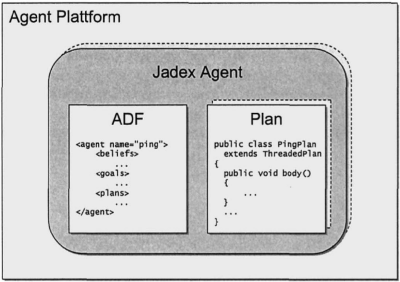
\includegraphics[scale=0.45]{figuras/jadex2.png}
\end{figure}

O JADEX � executado sobre a plataforma do JADE. A integra��o ocorre atrav�s de uma ferramenta de integra��o desenvolvida para injetar os agentes JADEX dentro do banco de agentes do JADE. Estes agentes s�o instanciados atrav�s de modelos criados a partir de seus arquivos descritores e seus comportamentos s�o mapeados como \emph{cyclic behaviours}, uma forma de comportamento dispon�vel provido pela plataforma JADE. Dessa forma, os planos s�o executados passo a passo e mant�m acesso sobre todas as caracter�sticas do agente. O JADEX acaba servindo como uma extens�o para a plataforma JADE, complementando-a com a possibilidade de especificar agentes cognitivos complexos que usam a estrat�gia de BDI para tomada de decis�es.


\subsubsection{JASON}

\textit{JASON} � um interpretador para uma vers�o estendida da linguagem de programa��o abstrata \textit{AgentSpeak} desenvolvido por \cite{bordini2007programming} utilizando a linguagem \textit{Java} e distribu�do pela licensa LGPL \cite{jasonsite}. O \textit{JASON}, al�m de implementar a sem�ntica operacional da linguagem, providencia uma plataforma para o desenvolvimento de sistemas multiagente, que suporta tanto o desenvolvimento de agentes reativos, quanto o de agentes baseados na arquitetura \textit{BDI}. Dentre as funcionalidades oferecidas pela plataforma \textit{JASON}, vale citar:

\begin{itemize}
	\item Nega��o forte: permite modelos de mundos abertos e fechados;
	\item Tratamento de falhas nos planos dos agentes;
	\item Comunica��o entre agentes baseada em atos de fala;
	\item Meta-eventos e nota��es declarativas de metas de agentes;
	\item Interoperabilidade com a ferramenta JADE. � poss�vel criar agentes \textit{JASON} que podem participar de um sistema multiagente operado pelo JADE, tanto quanto utilizar a estrutura da plataforma JADE para executar um sistema multiagente da plataforma \textit{JASON} de forma distribu�da em uma rede.
\end{itemize}

